\documentclass[pdf]{beamer}

\mode<presentation>{\usetheme{Warsaw}}
\usecolortheme{dove}

% http://web.mit.edu/rsi/www/pdfs/beamer-tutorial.pdf
% https://rohanverma.net/blog/2017/12/20/setting-up-latex-on-spacemacs/
% begin end CTRL-c CRTL-e

\AtBeginSection[]
{
\begin{frame}
    \frametitle{Contents}
    \tableofcontents[currentsection, hideothersubsections]
\end{frame}
}

% many duplicates, needs refactoring
\usepackage[notocbib]{apacite} % This does not put the bibliography in the table of contents if it is an unnumbered section or chapter. 
\bibliographystyle{apacite}
\nobibintoc % only works for apacite
\renewcommand\bibsection{\section[]{\refname}}

\usepackage[defaultfam,tabular,lining]{montserrat} %% Option 'defaultfam'

\usepackage[numbers]{natbib}
\newcommand\Fontvi{\fontsize{6}{7.2}\selectfont}

%% only if the base font of the document is to be sans serif
\usepackage[T1]{fontenc}
\usepackage{graphicx}
\renewcommand*\oldstylenums[1]{{\fontfamily{Montserrat-TOsF}\selectfont #1}}

\definecolor{ao(english)}{rgb}{0.0, 0.6, 0.0} % warning: duplicate below
\definecolor{azure(colorwheel)}{rgb}{0.0, 0.5, 1.0} % warning: duplicate below
\definecolor{darkgray}{rgb}{0.4, 0.4, 0.4}
\newcommand{\entity}[1]{\textcolor{ao(english)}{#1}}
\newcommand{\intent}[1]{\textcolor{azure(colorwheel)}{#1}}
\newcommand{\demo}[1]{\textit{\textcolor{darkgray}{#1}}}

\newcommand{\pgreen}[1]{\color<#1>[rgb]{0.0, 0.6. 0.0}}
\newcommand{\pblue}[1]{\color<#1>[rgb]{0.0, 0.6, 1.0}}

\title{Automatically responding to customers}
\begin{document}

    \begin{frame}
        \titlepage
    \end{frame}

    \begin{frame}
        \frametitle{Table of Contents}
        \tableofcontents[hideothersubsections]
    \end{frame}

    \section{Introduction}
    \subsection{Research question 1}
    \begin{frame}{Existing benchmarks}
        \begin{itemize}
            \item Braun et al.~\cite{braun2017}
            \item Snips~\cite{snips2017benchmarking} (next slide)
            \item Burtsev et al.~\cite{burtsev2018}
            \item Botfuel~\cite{botfuel2018benchmark}
        \end{itemize}
    \end{frame}

    \begin{frame}{Snips entity recognition}
        \begin{center}
            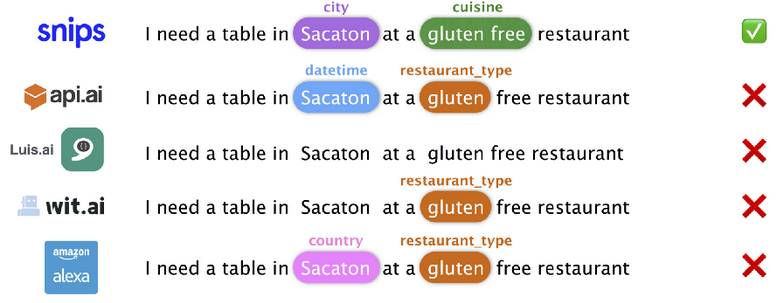
\includegraphics[width=\textwidth]{figures/snips_ner.png}
        \end{center}
    \end{frame}

    \begin{frame}{Their results}
        \begin{center}
            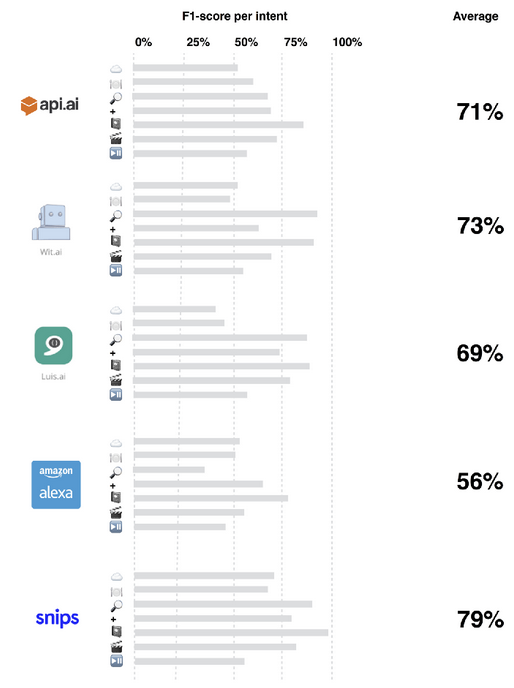
\includegraphics[height=0.85\textheight]{figures/snips_own_benchmark.png}
        \end{center}
    \end{frame}

    \begin{frame}{Question and goal}
        \begin{itemize}
            \item Can an open-source NLU benchmarking tool be created?
            \item Develop such a tool.
        \end{itemize}
    \end{frame}

    \subsection{Research question 2}
    \begin{frame}{Improving accuracy}
        How hard can it be?
    \end{frame}

    \begin{frame}{Question and goal}
        \begin{itemize}
            \item Can the accuracy for NLU be increased?
            \item Improve the accuracy
        \end{itemize}
    \end{frame}


    \section{Preliminaries}
    \subsection{Natural language processing}
    \begin{frame}{Description of NLP field}
        \begin{itemize}
            \item Extract meaningful information from text or speech
            \item Generate text or speech
        \end{itemize}
    \end{frame}

    \begin{frame}{Some well-known NLP tasks}
        \begin{itemize}
            \item Machine translation
            \item Speech recognition
            \item {\pgreen{2-3}{Named-entity recognition (NER)}}
            \item {\pblue{3}{Intent classification}}
        \end{itemize}
        \vspace*{5mm}
        \uncover<2-3>{\demo{What is [London's](\entity{location}) weather [tomorrow](\entity{date})?}} \\[3mm]
        \uncover<3>{\demo{\intent{GetWeather}}}
    \end{frame}
    \begin{frame}{Language model}
        \begin{itemize}
            \item Rule-based
            \end{itemize}
        \begin{itemize}
            \item Statistical\\[3mm]
        \end{itemize}
        \uncover<2>{
        Tries to capture grammar\\[1mm]
        \vspace*{5mm}
        \begin{tabular}{l l}
            \textbf{Task} & \textbf{Example}\\
            \hline
            Spell correction & $P(\text{\demo{my car broke}}) > P(\text{\demo{my car boke}})$\\
            Machine translation & $P(\text{\demo{green house}}) > P(\text{\demo{house green}})$\\
            Speech recognition & $P(\text{\demo{the red car}}) > P(\text{\demo{she read ar}})$
        \end{tabular}
        }
    \end{frame}

    \begin{frame}{Count-based}
      
    \end{frame}

    \subsection{Deep learning}
    { % all template changes are local to this group.
    \setbeamertemplate{navigation symbols}{}
    \begin{frame}[plain]
        \hspace*{-6cm}
        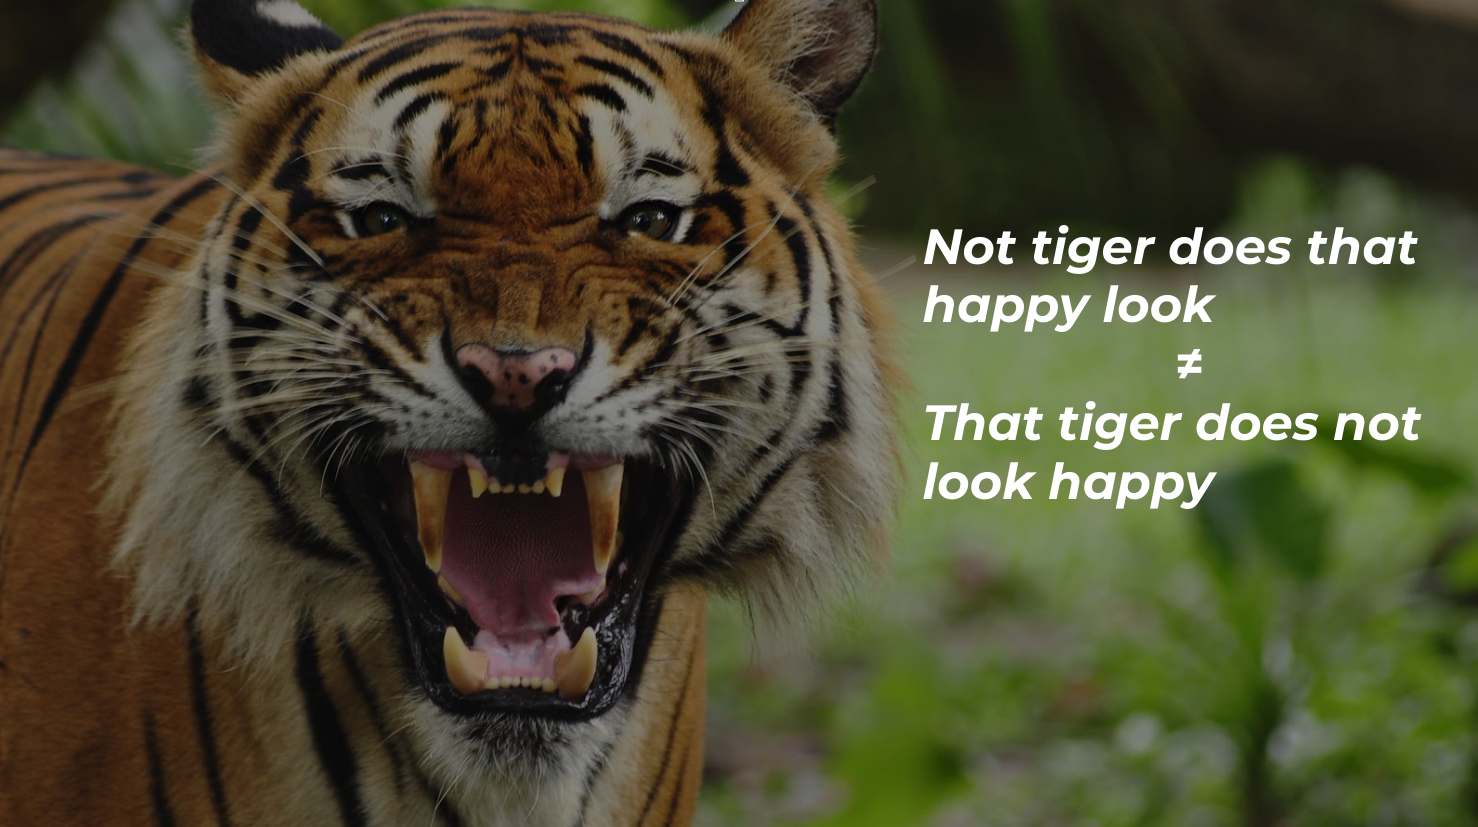
\includegraphics[scale=0.35]{figures/tiger.png}
    \end{frame}
    }

    \begin{frame}{Recurrent neural networks}
        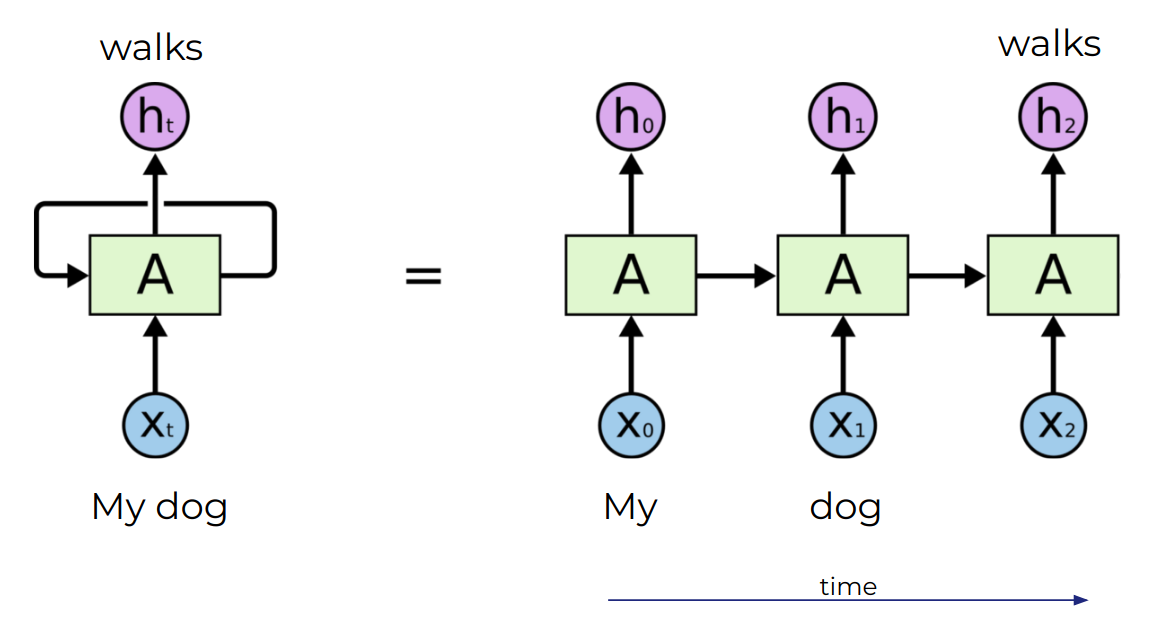
\includegraphics[width=\textwidth]{figures/rnn.png}
    \end{frame}

    \begin{frame}{Translating}
        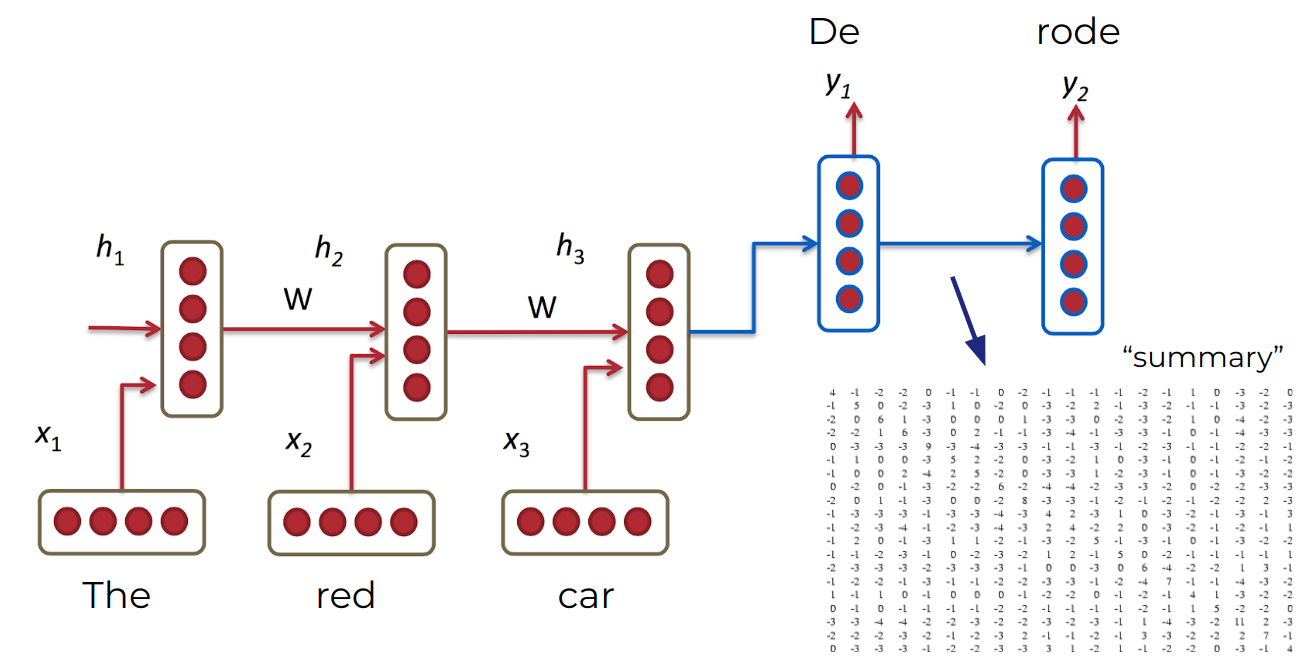
\includegraphics[width=\textwidth]{figures/encoder-decoder.png}
    \end{frame}

    \begin{frame}{Insufficient history}
        \begin{center}
            \demo{Norwegian \underline{frigate} sinking has far-reaching implications.}
        \end{center}
        \begin{center}
            \demo{Het zinken van het Noorse \underline{fregat} heeft verstrekkende gevolgen.}
        \end{center}
    \end{frame}

    \begin{frame}{Gated recurrent neural networks}
        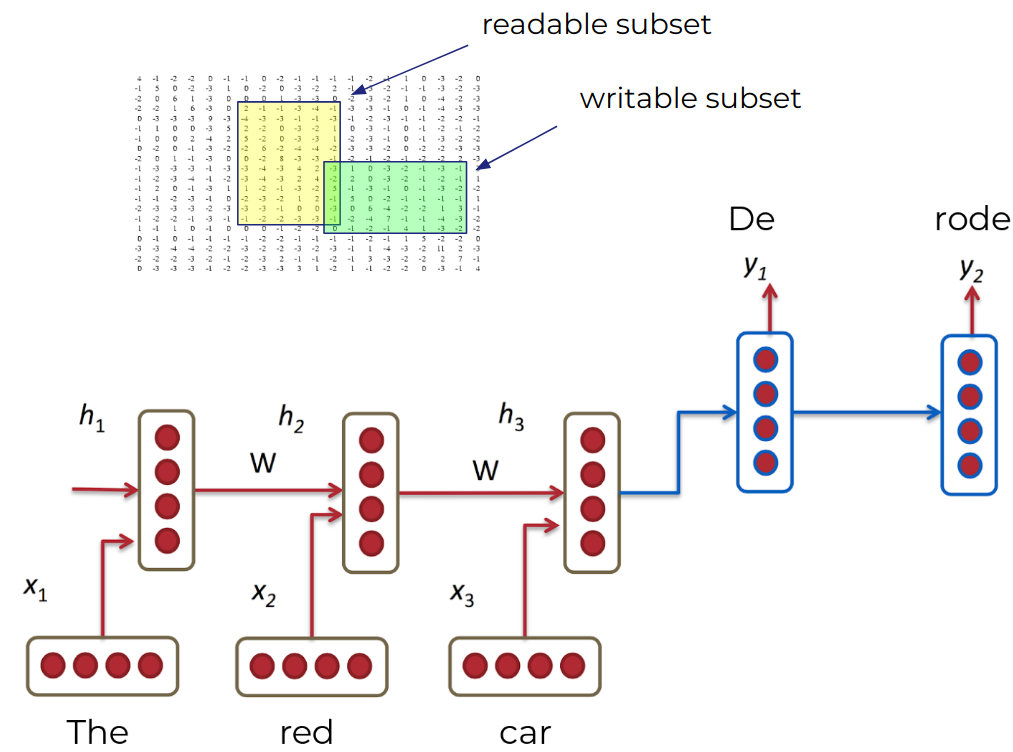
\includegraphics[height=0.9\textheight]{figures/gru.png}
    \end{frame}
    \section{Benchmarking}
    \subsection{Datasets}
    \begin{frame}{Overview}
        \begin{tabular}{l l l l l}
            \textbf{Dataset} & \textbf{Train} & \textbf{Test} & \textbf{\intent{Intents}} & \textbf{\entity{Entities}}\\
            \hline
            WebApplications & 30 & 54 & 7 & 1\\

            Chatbot & 100 & 106 & 2 & 5\\
            Snips2017 & 2100 & 700 & 7 & unknown\\
        \end{tabular}
    \end{frame}

    \begin{frame}{Example sentences}
        \begin{itemize}
            \item WebApplications\\
            \demo{How can I delete my [Hunch](\entity{WebService}) account?} \\
            \demo{\intent{DeleteAccount}}
            \item Chatbot \\
            \demo{when is the [next](\entity{criterion}) [train](\entity{vehicle}) in
            [muncher freiheit](\entity{StationStart})?} \\
            \demo{\intent{DepartureTime}}
            \item Snips2017 \\
            \demo{i want to listen to [Say it Again](\entity{track}) by
            [Blackstratblues](\entity{artist})} \\
            \demo{\intent{PlayMusic}}
        \end{itemize}
    \end{frame}

    \subsection{Systems}

    \begin{frame}{Rasa}
        \begin{columns}
            \column{0.5\textwidth}
            \begin{itemize}
                \item open-source
                \item free
                \item local instance
            \end{itemize}
            \column{0.5\textwidth}
            \begin{center}
                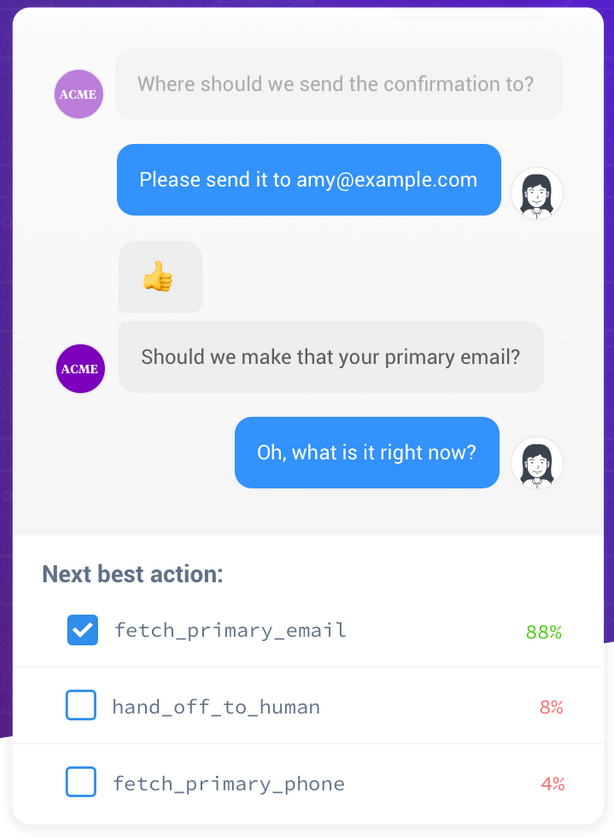
\includegraphics[height=0.9\textheight]{figures/rasa.png}
            \end{center}
        \end{columns}
    \end{frame}

    \begin{frame}{Rasa training data format}
        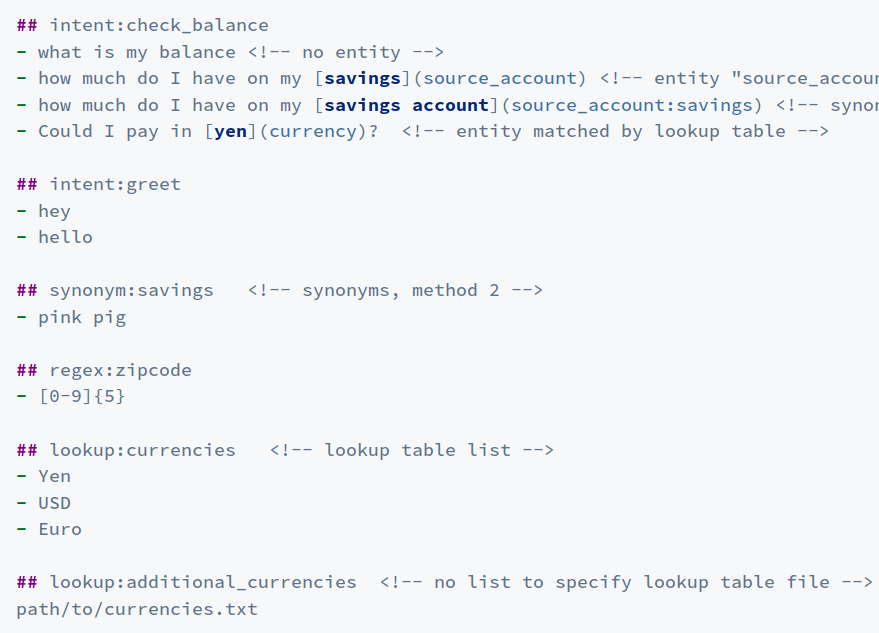
\includegraphics[width=\textwidth]{figures/rasa_data_format.png}
    \end{frame}

    \begin{frame}{IBM Watson Conversation}
        \hspace*{-1cm}
        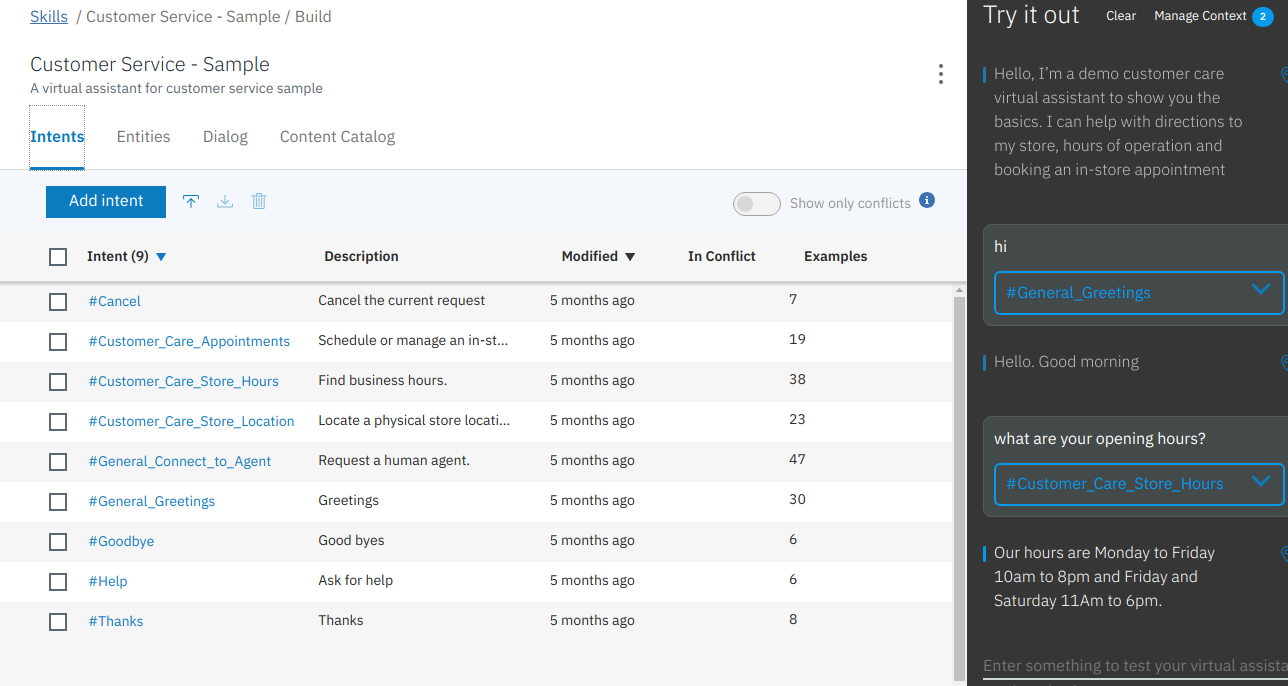
\includegraphics[height=0.9\textheight]{figures/watson.png}
    \end{frame}

    \subsection{Tool and results}
    \begin{frame}{Tool: \textsc{Bench}}
        \begin{itemize}
            \item Python
            \item Docker
            \item Not object-oriented\footnotemark
        \end{itemize}
        \footnotetext[1]{Steven Lott, Functional Python Programming}
      \end{frame}
      
    \begin{frame}{Results}
        \hspace*{-6mm}
        \begin{tabular}{l c c c c}
            \textbf{System} & \textbf{Source} & \textbf{Ask-} & \textbf{Chatbot} & \textbf{Web-} \\
            & & \textbf{Ubuntu} & & \textbf{Apps} \\
            \hline
            Rasa:0.5-mitie & Braun et al. & 0.862 & 0.981 & 0.746 \\
            Microsoft LUIS & Braun et al. & 0.899 & 0.981 & 0.814 \\
            Watson & Braun et al. & 0.917 & 0.972 & 0.831 \\
            Rasa:0.13.7-mitie & \textsc{bench} & 0.881 & & 0.763 \\
            Rasa:0.13.8-spacy & \textsc{bench} & 0.853 & 0.981 & 0.627 \\
            Watson & \textsc{bench} & 0.881 & 0.934 & 0.831 \\
            \hline
        \end{tabular}
    \end{frame}

    \section{Improving accuracy}

    \subsection{BERT}
    \begin{frame}{Overview}
        \begin{itemize}
            \item December 2018
            \item SOTA 11 tasks\\[5mm]

            \item Transformer (less sequential and $\mathcal{O} (1)$ history)
            \item Pre-training
            \item Deep bidirectionality
        \end{itemize}
    \end{frame}

    \begin{frame}{Deep bidirectionality}
        \begin{center}
            \begin{tabular}{c c c c c}
                \demo{the} & \demo{...} & \demo{on} & \demo{the} & \demo{hill} \\
                $T_1$ & $T_2$ & $T_4$ & $T_5$ & $T_6$
            \end{tabular}
        \end{center}

        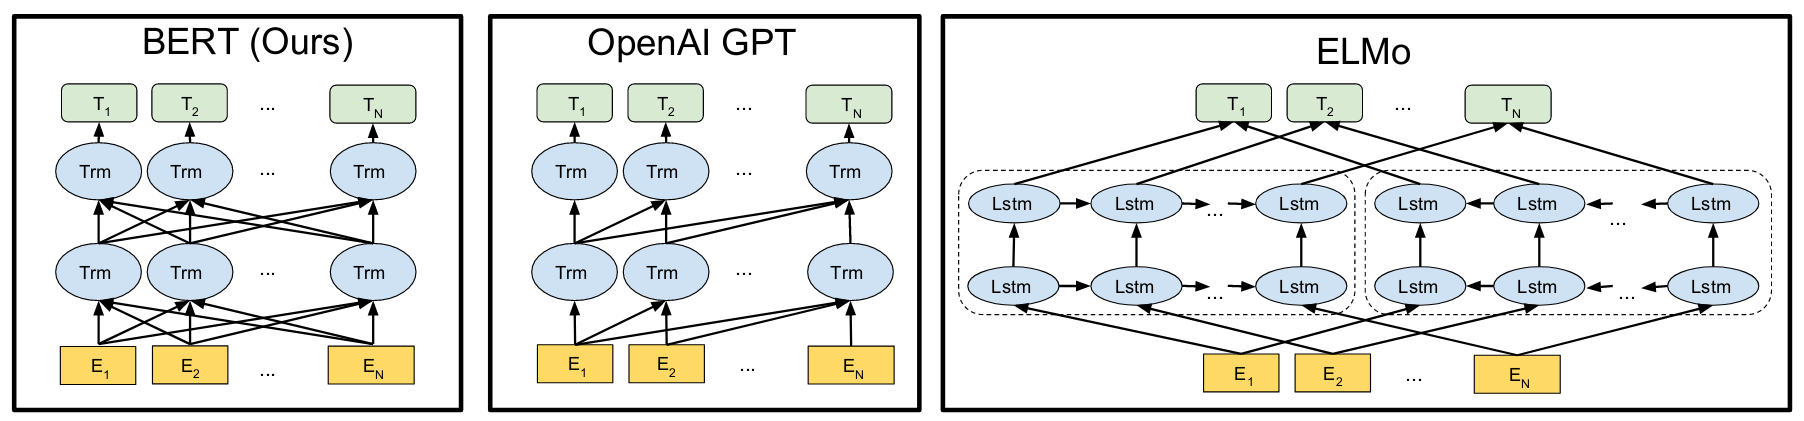
\includegraphics[width=\textwidth]{../figures/deeply_bidirectional.png}
    \end{frame}

    \subsection{Training}
    \begin{frame}{Single sentence classification}
        \begin{columns}
            \column{0.7\textwidth}
            \begin{center}
                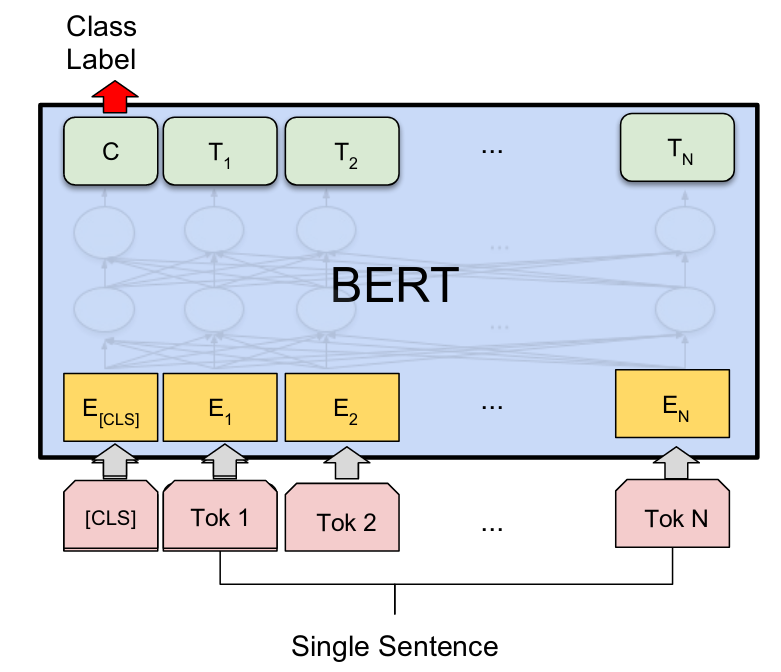
\includegraphics[height=0.87\textheight]{../figures/bert_single_sentence.png}
            \end{center}
            \column{0.3\textwidth}
            \begin{itemize}
                \item Training time: 1.5 days
                \item Occasional near zero accuracy
            \end{itemize}
        \end{columns}
    \end{frame}

    \begin{frame}{Sequential labelling}
        \vspace*{-1cm}
         \begin{columns}
            \column{0.7\textwidth}
            \begin{center}
                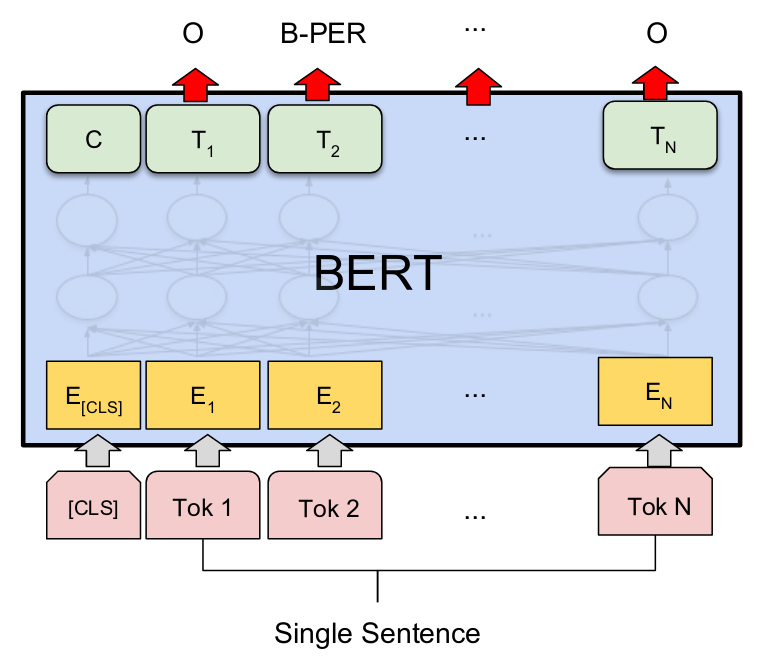
\includegraphics[height=0.87\textheight]{../figures/bert_ner.png}
            \end{center}
            \column{0.3\textwidth}
             \begin{itemize}
                \item NER SOTA
            \end{itemize}
        \end{columns}
    \end{frame}

    \subsection{Joint training}
    \begin{frame}{Intuition}
        \intent{GetWeather}: \\[5mm]

        \demo{Will it rain in \entity{London} \entity{tomorrow}?}  \\
        \demo{What is the \entity{today's} temperature in \entity{Madrid}?} \\[5mm]

        \demo{Will it rain in \entity{$<$location$>$} \entity{$<$date$>$}?} \\
        \demo{What is the \entity{$<$date$>$} temperature in \entity{$<$location$>$}?}
    \end{frame}

    \subsection{Results}
    \begin{frame}{F$_1$ scores}
        \hspace*{-7mm}
        \begin{tabular}{l l l l l c c}
        \textbf{Dataset}    & \textbf{Steps} & \textbf{Method}   & \textbf{\intent{Intent}}  & \textbf{\entity{Entity}}\\
        \hline
        Web-                & & Rasa & $0.67 \pm 0.04$\\
        Apps                & 600 (twice) & separate & $0.72 \pm 0.03$ & $0.81 \pm 0.01$ \\
                            & \uncover<2>{600 & joint & $0.76 \pm 0.07$ & $0.82 \pm 0.01$} \\
        \hline
        Ask-                & & Rasa & $0.84 \pm 0.00$ \\
        Ubuntu              & 600 (twice) & separate & $0.82 \pm 0.05$ & $0.81 \pm 0.01$\\
                            & \uncover<2>{600 & joint & $0.87 \pm 0.01$ & $0.83 \pm 0.00$} \\
        \hline
        Chatbot             & & Rasa & $0.98 \pm 0.00$ \\
                            & 600 (twice) & separate & $0.84 \pm 0.21$ & $0.76 \pm 0.00$\\
                            & \uncover<2>{600 & joint & $0.98 \pm 0.00$ & $0.79 \pm 0.00$} \\
        \hline
        Snips-              & & Rasa & $0.99 \pm 0.00$\\
        2017                & 6000 (twice) & separate & $0.04 \pm 0.00$ & $0.84 \pm 0.00$\\
                            & \uncover<2>{6000 & joint & $0.98 \pm 0.02$ & $0.86 \pm 0.00$} \\
        \hline
    \end{tabular}
    \end{frame}

    \begin{frame}{Future work}
        \begin{itemize}
            \item Code validation
            \item Loss function
            \item Entities baseline comparison
            \item Datasets
            \item `Mobile friendly' transformer\footnotemark
        \end{itemize}
        \footnotetext[2]{So et al., The Evolved Transformer (30 jan 2019)}
    \end{frame}

    \section{Conclusions}
    \subsection{Research question 1}
    \begin{frame}{Can an open-source NLU benchmarking tool be created?}
        Yes.
        Requirements:
        \begin{itemize}
            \item Continuous maintenance
            \item Support vendor APIs
            \item More metrics
            \item Multiple runs
            \item More datasets
        \end{itemize}
    \end{frame}

    \subsection{Research question 2}
    \begin{frame}{Can the accuracy for NLU be increased?}
        Yes.
        Each few months a new SOTA paper.\\[5mm]

        Why BERT is suspected to have improved SOTA:
        \begin{itemize}
            \item SOTA NER
            \item Deeply bidirectional
            \item More history.\\[5mm]
        \end{itemize}

        Further work: Whether accuracy improvements are significant.
    \end{frame}

   \begin{frame}[allowframebreaks]{References}
        \scriptsize
        % \bibliographystyle{plainnat}
        \bibliography{../references.bib}
\end{frame}

\end{document}